\documentclass{article}
\usepackage[T1]{fontenc}
\usepackage[utf8]{inputenc}
\usepackage[swedish]{babel}
\usepackage{amsmath, amssymb, mathtools}
\usepackage{enumitem}
\usepackage{siunitx}
\usepackage{listings}
\usepackage{comment}
\usepackage{tikz, pgfplots}
\usepackage{afterpage}
\usepackage{booktabs}

\makeatletter
\def\fps@figure{hbtp}
\def\fps@table{hbtp}
\makeatother

\pgfplotsset{compat=newest}
\sisetup{
	round-mode      = places,
	round-precision = 3
	}

\lstset{
	breaklines=true,
	postbreak=\mbox{\textcolor{red}{$\hookrightarrow$}\space},
	}

\DeclareMathOperator\Beta{Beta}
\DeclareMathOperator\Poisson{Pois}
\DeclareMathOperator\GammaDist{Gamma}
\DeclareMathOperator\BetaDist{Beta}
\DeclareMathOperator\Normal{Normal}
\DeclareMathOperator\NegBin{Neg-Bin}
\DeclareMathOperator\Uniform{Uniform}
\newcommand{\size}[1]{\lvert #1 \rvert}

\title{Third Assignment in MVE550}
\author{Axel Forsman, Jonas Lauri}

\begin{document}
\maketitle

\section{Question 1}
Imagine we have square of dimensions $[0,1] \times [0,1]$ with 36 trees.
\begin{enumerate}[label=(\alph*)]
	\item A modeling of the trees can be seen as a spatial Poisson process with parameter $\lambda = 36$. Compute the probability of 6 or more trees in the area $[0.2, 0.6] \times [0.2, 0.6]$.
	\item With the same assumptions, compute the probability of exactly 4 trees in $[0.2, 0.6] \times [0.2, 0.6]$ AND exactly 4 trees in $[0.4, 0.8] \times [0.4, 0.8]$.
	\item With the same assumptions, write R code as to simulate this spatial process and show one such simulation.
	\item Assume that $\lambda$ has the prior $\pi(\lambda) \propto_\lambda 1/\lambda$ and we have observed 36 trees in the square $[0,1] \times [0,1]$. Derive the posterior for $\lambda$. Use this posterior in (c) to simulate.
	\item With the stochastic process simulated in (d), derive the average of the distance to the nearest neighbour. Let this be $X$. Then, for $k$ points,
	$$X = \frac{1}{k}\sum_{i=1}^k \min_{j = 1, ..., k} \sqrt{(x_i-x_j)^2+(y_i-y_j)^2)}, j \neq i.$$
	Simulate a couple $X$ and plot the distribution.
	\item From the real life data $X = 0.1358$. Use the result from (e) to discuss if the Poisson model is good, and if not what should be changed.
	\item With the process in (d), consider $Y$ a random variable representing the number of points in the circle centered at (0.5, 0.5) with radius 0.1. Determine the name and the parameters of the $Y$ distribution.
\end{enumerate}

\subsection{(a)}
$(N_A)_{A \subseteq \mathbb R^2}$ is a spatial Poisson process
with parameter $\lambda = 36$.
Let $A \coloneqq [0.2, 0.6] \times [0.2, 0.6] \subseteq \mathbb R^2$.
Then $N_A$ has a Poisson distribution with parameter $\lambda \lvert A \rvert$.
Whence we get
$$ \mathbb P(N_A \ge 6) = 1 - \mathbb P(N_A \le 5) = 1 - \Poisson(5; 36 \cdot 0.4^2)
\approx \num{0.5150434} $$

\subsection{(b)}
\begin{center}
	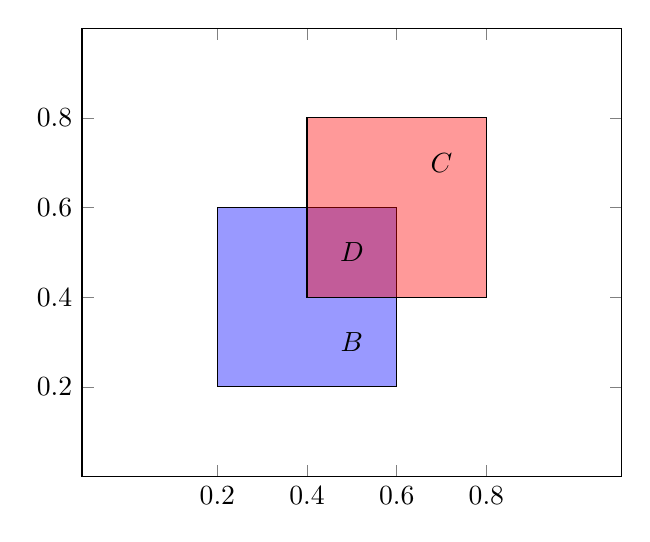
\begin{tikzpicture}
		\begin{axis}[xmin = 0, xmax = 1, ymin=0, ymax = 1, axis equal,
			xtick = {0.2, 0.4, 0.6, 0.8}, ytick = {0.2, 0.4, 0.6, 0.8},
			clip = false]
			\fill[blue, fill opacity=0.4, draw=black] (0.2, 0.2) rectangle (0.6, 0.6);
			\fill[red, fill opacity=0.4, draw=black] (0.8, 0.8) rectangle (0.4, 0.4);
			\node at (0.5, 0.3) {$B$};
			\node at (0.7, 0.7) {$C$};
			\node at (0.5, 0.5) {$D$};
		\end{axis}
	\end{tikzpicture}
\end{center}

Let $B \coloneqq A \setminus D, C \coloneqq A \setminus D, D \coloneqq [0.4, 0.6]^2$.
Then
\begin{align*}
	\mathbb P(N_{B \cup D = 4}, N_{C \cup D = 4}) &= \sum_{k=0}^4 \mathbb P(N_D = k) \underbrace{\mathbb P(N_{B \cup D} = 4, N_{C \cup D} = 4 \mid N_D = k)}_{\mathbb P(N_B = 4 - k, N_C = 4 - k)} \\
												  &= \sum_{k=0}^4 \mathbb P(N_D = k) \mathbb P(N_B = 4 - k) \mathbb P(N_C = 4 - k) \\
												  &= \sum_{k=0}^4 \Poisson(k; \lambda \size{D}) \Poisson(4 - k; \lambda \size{B})^2
												  \approx \num{0.023902}
\end{align*}
where we have used that $N_B, N_C$ are independent since $B, C$ are disjoint.

\subsection{(c)}
Since conditional on the number of points in $A \coloneqq [0, 1]^2$,
the positions of the points are uniformly distributed in $A$,
we can simulate such a process using
\begin{lstlisting}[language = R]
N <- rpois(1, lambda * 1^2)
list(x = runif(N, 0, 1), y = runif(N, 0, 1))
\end{lstlisting}
One such example simulation is shown in figure~\ref{fig:c_sim}.

\begin{figure}
	\centering
	% Created by tikzDevice version 0.12.3 on 2019-12-19 15:29:19
% !TEX encoding = UTF-8 Unicode
\begin{tikzpicture}[x=1pt,y=1pt]
\definecolor{fillColor}{RGB}{255,255,255}
\path[use as bounding box,fill=fillColor,fill opacity=0.00] (0,0) rectangle (289.08,289.08);
\begin{scope}
\path[clip] ( 67.20, 61.20) rectangle (245.88,239.88);
\definecolor{drawColor}{RGB}{0,0,0}

\path[draw=drawColor,line width= 0.4pt,line join=round,line cap=round] (236.20, 96.22) --
	(239.23, 90.97) --
	(233.17, 90.97) --
	(236.20, 96.22);

\path[draw=drawColor,line width= 0.4pt,line join=round,line cap=round] (210.65,113.67) --
	(213.68,108.42) --
	(207.62,108.42) --
	(210.65,113.67);

\path[draw=drawColor,line width= 0.4pt,line join=round,line cap=round] (135.50, 88.91) --
	(138.53, 83.66) --
	(132.47, 83.66) --
	(135.50, 88.91);

\path[draw=drawColor,line width= 0.4pt,line join=round,line cap=round] (155.24,188.04) --
	(158.27,182.79) --
	(152.21,182.79) --
	(155.24,188.04);

\path[draw=drawColor,line width= 0.4pt,line join=round,line cap=round] ( 79.46, 94.68) --
	( 82.49, 89.43) --
	( 76.43, 89.43) --
	( 79.46, 94.68);

\path[draw=drawColor,line width= 0.4pt,line join=round,line cap=round] (168.71,227.72) --
	(171.74,222.47) --
	(165.68,222.47) --
	(168.71,227.72);

\path[draw=drawColor,line width= 0.4pt,line join=round,line cap=round] (148.70, 89.39) --
	(151.73, 84.14) --
	(145.67, 84.14) --
	(148.70, 89.39);

\path[draw=drawColor,line width= 0.4pt,line join=round,line cap=round] ( 79.22,193.04) --
	( 82.25,187.79) --
	( 76.19,187.79) --
	( 79.22,193.04);

\path[draw=drawColor,line width= 0.4pt,line join=round,line cap=round] ( 77.91,117.15) --
	( 80.95,111.90) --
	( 74.88,111.90) --
	( 77.91,117.15);

\path[draw=drawColor,line width= 0.4pt,line join=round,line cap=round] (130.83, 93.68) --
	(133.86, 88.43) --
	(127.80, 88.43) --
	(130.83, 93.68);

\path[draw=drawColor,line width= 0.4pt,line join=round,line cap=round] (163.10,143.97) --
	(166.13,138.72) --
	(160.07,138.72) --
	(163.10,143.97);

\path[draw=drawColor,line width= 0.4pt,line join=round,line cap=round] (209.84, 87.27) --
	(212.87, 82.02) --
	(206.81, 82.02) --
	(209.84, 87.27);

\path[draw=drawColor,line width= 0.4pt,line join=round,line cap=round] (165.13,122.03) --
	(168.16,116.79) --
	(162.10,116.79) --
	(165.13,122.03);

\path[draw=drawColor,line width= 0.4pt,line join=round,line cap=round] (208.73,167.78) --
	(211.76,162.54) --
	(205.70,162.54) --
	(208.73,167.78);

\path[draw=drawColor,line width= 0.4pt,line join=round,line cap=round] (146.72,169.72) --
	(149.75,164.47) --
	(143.69,164.47) --
	(146.72,169.72);

\path[draw=drawColor,line width= 0.4pt,line join=round,line cap=round] ( 76.06,147.68) --
	( 79.09,142.43) --
	( 73.03,142.43) --
	( 76.06,147.68);

\path[draw=drawColor,line width= 0.4pt,line join=round,line cap=round] (173.85, 71.49) --
	(176.88, 66.24) --
	(170.82, 66.24) --
	(173.85, 71.49);

\path[draw=drawColor,line width= 0.4pt,line join=round,line cap=round] ( 78.94,111.98) --
	( 81.97,106.73) --
	( 75.91,106.73) --
	( 78.94,111.98);

\path[draw=drawColor,line width= 0.4pt,line join=round,line cap=round] (104.43,157.34) --
	(107.46,152.09) --
	(101.40,152.09) --
	(104.43,157.34);

\path[draw=drawColor,line width= 0.4pt,line join=round,line cap=round] (234.32,171.94) --
	(237.35,166.70) --
	(231.29,166.70) --
	(234.32,171.94);

\path[draw=drawColor,line width= 0.4pt,line join=round,line cap=round] (232.61,208.24) --
	(235.64,202.99) --
	(229.58,202.99) --
	(232.61,208.24);

\path[draw=drawColor,line width= 0.4pt,line join=round,line cap=round] (128.69,156.16) --
	(131.72,150.92) --
	(125.66,150.92) --
	(128.69,156.16);

\path[draw=drawColor,line width= 0.4pt,line join=round,line cap=round] (103.54,211.82) --
	(106.57,206.57) --
	(100.51,206.57) --
	(103.54,211.82);

\path[draw=drawColor,line width= 0.4pt,line join=round,line cap=round] (146.87,184.67) --
	(149.90,179.42) --
	(143.84,179.42) --
	(146.87,184.67);

\path[draw=drawColor,line width= 0.4pt,line join=round,line cap=round] (235.47, 74.21) --
	(238.50, 68.96) --
	(232.44, 68.96) --
	(235.47, 74.21);

\path[draw=drawColor,line width= 0.4pt,line join=round,line cap=round] ( 77.90,228.23) --
	( 80.93,222.99) --
	( 74.87,222.99) --
	( 77.90,228.23);

\path[draw=drawColor,line width= 0.4pt,line join=round,line cap=round] (138.05,113.04) --
	(141.08,107.79) --
	(135.02,107.79) --
	(138.05,113.04);

\path[draw=drawColor,line width= 0.4pt,line join=round,line cap=round] ( 82.87, 85.26) --
	( 85.90, 80.02) --
	( 79.84, 80.02) --
	( 82.87, 85.26);

\path[draw=drawColor,line width= 0.4pt,line join=round,line cap=round] ( 75.15,120.52) --
	( 78.18,115.27) --
	( 72.12,115.27) --
	( 75.15,120.52);

\path[draw=drawColor,line width= 0.4pt,line join=round,line cap=round] (176.73,178.43) --
	(179.76,173.18) --
	(173.70,173.18) --
	(176.73,178.43);

\path[draw=drawColor,line width= 0.4pt,line join=round,line cap=round] (168.97, 81.33) --
	(172.00, 76.08) --
	(165.94, 76.08) --
	(168.97, 81.33);

\path[draw=drawColor,line width= 0.4pt,line join=round,line cap=round] (139.87,124.87) --
	(142.90,119.62) --
	(136.84,119.62) --
	(139.87,124.87);

\path[draw=drawColor,line width= 0.4pt,line join=round,line cap=round] ( 87.45,172.32) --
	( 90.48,167.07) --
	( 84.42,167.07) --
	( 87.45,172.32);

\path[draw=drawColor,line width= 0.4pt,line join=round,line cap=round] (238.66,220.55) --
	(241.69,215.30) --
	(235.63,215.30) --
	(238.66,220.55);

\path[draw=drawColor,line width= 0.4pt,line join=round,line cap=round] (193.74, 73.65) --
	(196.77, 68.40) --
	(190.71, 68.40) --
	(193.74, 73.65);

\path[draw=drawColor,line width= 0.4pt,line join=round,line cap=round] (170.53, 93.79) --
	(173.56, 88.54) --
	(167.50, 88.54) --
	(170.53, 93.79);

\path[draw=drawColor,line width= 0.4pt,line join=round,line cap=round] (103.26,195.47) --
	(106.29,190.22) --
	(100.23,190.22) --
	(103.26,195.47);

\path[draw=drawColor,line width= 0.4pt,line join=round,line cap=round] ( 93.12, 77.22) --
	( 96.15, 71.97) --
	( 90.09, 71.97) --
	( 93.12, 77.22);

\path[draw=drawColor,line width= 0.4pt,line join=round,line cap=round] (234.61, 86.16) --
	(237.65, 80.92) --
	(231.58, 80.92) --
	(234.61, 86.16);

\path[draw=drawColor,line width= 0.4pt,line join=round,line cap=round] (150.90, 80.83) --
	(153.93, 75.58) --
	(147.87, 75.58) --
	(150.90, 80.83);

\path[draw=drawColor,line width= 0.4pt,line join=round,line cap=round] (200.03, 90.72) --
	(203.06, 85.47) --
	(197.00, 85.47) --
	(200.03, 90.72);

\path[draw=drawColor,line width= 0.4pt,line join=round,line cap=round] (173.40,159.92) --
	(176.43,154.67) --
	(170.37,154.67) --
	(173.40,159.92);

\path[draw=drawColor,line width= 0.4pt,line join=round,line cap=round] (117.64,144.76) --
	(120.67,139.51) --
	(114.61,139.51) --
	(117.64,144.76);

\path[draw=drawColor,line width= 0.4pt,line join=round,line cap=round] ( 92.51,213.30) --
	( 95.54,208.06) --
	( 89.48,208.06) --
	( 92.51,213.30);

\path[draw=drawColor,line width= 0.4pt,line join=round,line cap=round] (192.24, 78.33) --
	(195.27, 73.08) --
	(189.20, 73.08) --
	(192.24, 78.33);

\path[draw=drawColor,line width= 0.4pt,line join=round,line cap=round] (131.40, 99.89) --
	(134.43, 94.65) --
	(128.37, 94.65) --
	(131.40, 99.89);

\path[draw=drawColor,line width= 0.4pt,line join=round,line cap=round] (145.82, 93.11) --
	(148.85, 87.86) --
	(142.79, 87.86) --
	(145.82, 93.11);
\end{scope}
\begin{scope}
\path[clip] (  0.00,  0.00) rectangle (289.08,289.08);
\definecolor{drawColor}{RGB}{0,0,0}

\path[draw=drawColor,line width= 0.4pt,line join=round,line cap=round] ( 73.82, 61.20) -- (239.26, 61.20);

\path[draw=drawColor,line width= 0.4pt,line join=round,line cap=round] ( 73.82, 61.20) -- ( 73.82, 55.20);

\path[draw=drawColor,line width= 0.4pt,line join=round,line cap=round] (106.91, 61.20) -- (106.91, 55.20);

\path[draw=drawColor,line width= 0.4pt,line join=round,line cap=round] (140.00, 61.20) -- (140.00, 55.20);

\path[draw=drawColor,line width= 0.4pt,line join=round,line cap=round] (173.08, 61.20) -- (173.08, 55.20);

\path[draw=drawColor,line width= 0.4pt,line join=round,line cap=round] (206.17, 61.20) -- (206.17, 55.20);

\path[draw=drawColor,line width= 0.4pt,line join=round,l);
\end{scope}
\end{tikzpicture}
\begin{tikzpicture}[x=1pt,y=1pt]
\definecolor{fillColor}{RGB}{255,255,255}
\path[use as bounding box,fill=fillColor,fill opacity=0.00] (0,0) rectangle (216.81,216.81);
\begin{scope}
\path[clip] (  0.00,  0.00) rectangle (216.81,216.81);
\definecolor{drawColor}{RGB}{0,0,0}

\node[text=drawColor,anchor=base,inner sep=0pt, outer sep=0pt, scale=  1.20] at (120.41,188.07) {\bfseries Histogram of Xs};

\node[text=drawColor,anchor=base,inner sep=0pt, outer sep=0pt, scale=  1.00] at (120.41, 15.60) {Xs};

\node[text=drawColor,rotate= 90.00,anchor=base,inner sep=0pt, outer sep=0pt, scale=  1.00] at ( 28.80,114.41) {Density};
\end{scope}
\begin{scope}
\path[clip] (  0.00,  0.00) rectangle (216.81,216.81);
\definecolor{drawColor}{RGB}{0,0,0}

\path[draw=drawColor,line width= 0.4pt,line join=round,line cap=round] ( 79.35, 61.20) -- (161.46, 61.20);

\path[draw=drawColor,line width= 0.4pt,line join=round,line cap=round] ( 79.35, 61.20) -- ( 79.35, 55.20);

\path[draw=drawColor,line width= 0.4pt,line join=round,line cap=round] ( 95.77, 61.20) -- ( 95.77, 55.20);

\path[draw=drawColor,line width= 0.4pt,line join=round,line cap=round] (112.19, 61.20) -- (112.19, 55.20);

\path[draw=drawColor,line width= 0.4pt,line join=round,line cap=round] (128.62, 61.20) -- (128.62, 55.20);

\path[draw=drawColor,line width= 0.4pt,line join=round,line cap=round] (145.04, 61.20) -- (145.04, 55.20);

\path[draw=drawColor,line width= 0.4pt,line join=round,line cap=round] (161.46, 61.20) -- (161.46, 55.20);

\node[text=drawColor,anchor=base,inner sep=0pt, outer sep=0pt, scale=  1.00] at ( 79.35, 39.60) {0.06};
\end{scope}
\end{tikzpicture}
;

\node[text=drawColor,rotate= 90.00,anchor=base,inner sep=0pt, outer sep=0pt, scale=  1.00] at ( 52.80,134.00) {0.4};

\node[text=drawColor,rotate= 90.00,anchor=base,inner sep=0pt, outer sep=0pt, scale=  1.00] at ( 52.80,167.08) {0.6};

\node[text=drawColor,rotate= 90.00,anchor=base,inner sep=0pt, outer sep=0pt, scale=  1.00] at ( 52.80,200.17) {0.8};

\node[text=drawColor,rotate= 90.00,anchor=base,inner sep=0pt, outer sep=0pt, scale=  1.00] at ( 52.80,233.26) {1.0};

\path[draw=drawColor,line width= 0.4pt,line join=round,line cap=round] ( 67.20, 61.20) --
	(245.88, 61.20) --
	(245.88,239.88) --
	( 67.20,239.88) --
	( 67.20, 61.20);
\end{scope}
\end{tikzpicture}

	\caption{One simulation of the spatial Poisson process. \label{fig:c_sim}}
\end{figure}

\subsection{(d)}
Improper prior $\pi(\lambda) \propto_\lambda 1/\lambda \propto_\lambda \GammaDist(0, 0)$
Likelihood: $\pi(\text{data} \mid \lambda) = \Poisson(\lambda \cdot 1^2)$.
Due to the Poisson-Gamma conjugacy: $\pi(\lambda \mid \text{data}) = \GammaDist(36, 1)$

\subsection{(e)}
One such random sample is shown in figure~\ref{fig:X_histogram}.

\begin{figure}
    \centering
    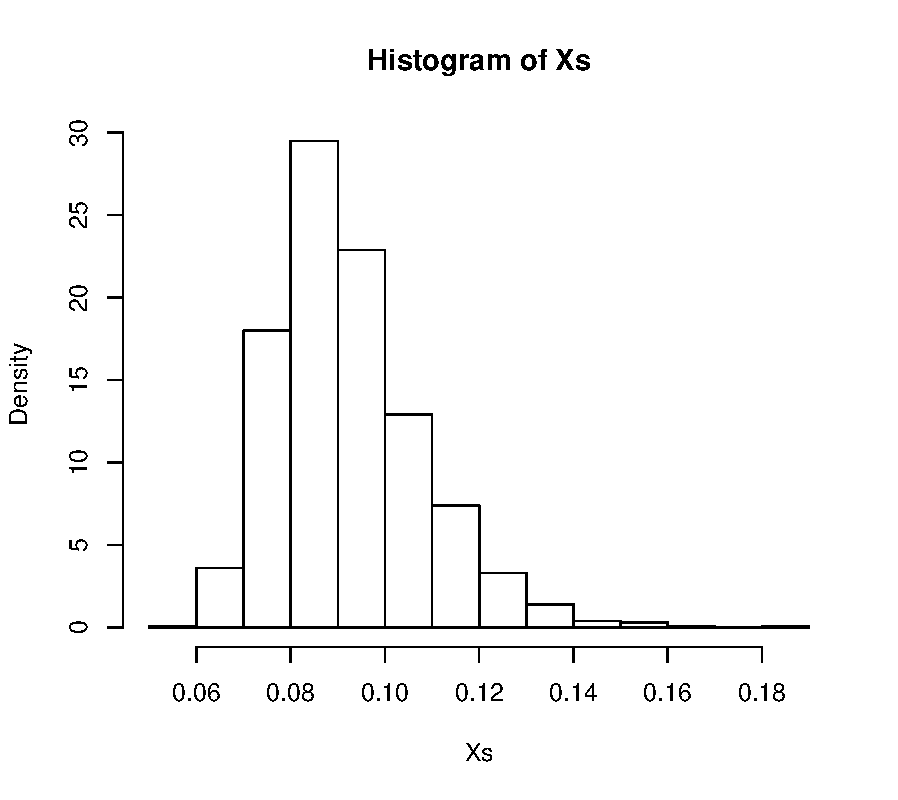
\includegraphics[scale = 0.7]{Histo_Xs.pdf}
	\caption{Histogram of the $X$:s. \label{fig:X_histogram}}
\end{figure}

\subsection{(f)}
In the results of (e) we get $Xs_{mean} \approx 0.092$ while for the example figure the $X = 0.136$.
The reason for this discrepancy between the $X$ is because of the nature of the Poisson distribution.
The probability of $n$ points in an area $A$ is equal to:
$$\frac{(\lambda |B|)^n}{n!}e^{-\lambda|B|} \propto_n \frac{(\lambda |B|)^n}{n!}$$
While this quickly goes to $0$ as $n$ increases, often two trees will overlap.
This causes $X$ to be drastically smaller than in the cases where there is no overlapping.
Two trees overlapping is of course an unlikely scenario because of physical limitations.
One way of changing the model would be to force new trees to separated from old ones.
This can be done by throwing away trees too close to already created ones.

\subsection{(g)}
We have that $Y \mid \lambda \sim \Poisson(\lambda \lvert D \rvert)$,
where $D$ is the disk of radius $0.1$ centered at $(0.5, 0.5)$,
$\lvert D \rvert = \pi 0.1^2$.
Since the posterior of $\lambda$ is known to be a Gamma distribution, using
$$ X \sim \GammaDist(\alpha, \beta) \implies cX \sim \GammaDist(\alpha, \frac\beta c) \quad \forall c>0 $$
we see that
$$ \frac{\size{D}}{\size{[0, 1]^2}} \lambda \mid \text{data} = \size{D} \lambda \mid \text{data}
\sim \GammaDist(36, \frac1{\size{D}}) $$
Due to Poisson and Gamma being conjugate distributions we get
$$ Y \mid \text{data} \sim \NegBin(36, 1 - \frac1{1 + \frac1{\size{D}}}) $$

\section{Question 2}
We have a contiuous-time, discrete state space Markov Chain with three states.
One run of the MC can be seen in the table below.
\begin{center}
\begin{tabular}{c|c|c|c|c|c|c|c|c|c|c|}
 State & 1 & 3 & 2 & 3 & 1 & 2 & 1 & 3 & 1 & 2 \\
 \hline
 Duration & 6.83 & 4.01 & 1.63 & 0.44 & 5.11 & 0.29 & 2.87 & 1.3 & 4.76 & 1.92
\end{tabular}
\end{center}
The vector for the holding times is: $q = (1/5, 1, 1/2)$.
The transition matrix for the embedded Markov chain is:
$$ \tilde{P} = \begin{bmatrix}
0 & 0.5 & 0.5\\
0.5 & 0 & 0.5\\
0.5 & 0.5 & 0
\end{bmatrix} $$
\begin{enumerate}[label=(\alph*)]
	\item Compute the generator matrix Q and the limiting distribution.
	\item We want to use the data in the table to learn about the chain. The independent priors are $\pi(q_1) \propto_{q_1} 1/q_1, \pi(q_2) \propto_{q_2} 1/q_2, \pi(q_3) \propto_{q_3} 1/q_3$ and for the rows of $\tilde{P}, p_{12} = p_{21} = p_{31} \sim \Beta(1/2, 1/2)$. What is the joint posterior distribution of $q_1, q_2, q_3, p_{12}, p_{21}, p_{31}.$
	\item Based on this posterior, simulate from the posterior infinitesimal generator matrix $Q$, and output and simulation.
\end{enumerate}

\subsection{(a)}
By multiplying the expected holding times, $q$,
with the probability of moving to each other state,
specified by $\tilde P$, we get:
$$ \hat{Q} = \begin{bmatrix}
0 & 0.1 & 0.1\\
0.5 & 0 & 0.5\\
0.25 & 0.25 & 0
\end{bmatrix}.$$
To get the generator matrix $Q$, we make sure each row sums to 0,
$$ Q = \begin{bmatrix}
-0.2 & 0.1 & 0.1\\
0.5 & -1 & 0.5\\
0.25 & 0.25 & -0.5
\end{bmatrix}.$$
To get the limiting distributions we take the matrix exponential with a high $t$.
$$ e^{50Q} = \begin{bmatrix}
0.625 & 0.125 & 0.25\\
0.625 & 0.125 & 0.25\\
0.625 & 0.125 & 0.25
\end{bmatrix}.$$

\subsection{(b)}
Since everything is independent we can compute posteriors seperately.
For the rows of $\tilde P$ we note that
$$ p_{ij} = \mathbb P(X_{k+1} = j \mid X_{k} = i), \quad ij \in {12, 21, 31} $$
Thus the likelihood becomes Bernoulli distributed.
Since Bernoulli and Beta are conjugate distributions
we from the for the three rows with
prior hyperparameters $\alpha = 1/2, \beta = 1/2$
the posterior hyperparameters
$$ \alpha_1 = \alpha + \sum^n x_i, \quad \beta_1 = \beta + n - \sum^n x_i $$
where $n$ are the number of times the chain was in the state in question,
and $x_i = 1$ if it moved to the corresponding state, $x_i = 0$ otherwise.
Thus
\begin{gather*}
	p_{12} \mid \text{data} \sim \Beta(\frac12 + 2, \frac12 + 4 - 2) = \Beta(\frac52, \frac52) \\
	p_{21} \mid \text{data} \sim \Beta(\frac12 + 1, \frac12 + 2 - 1) = \Beta(\frac32, \frac32) \\
	p_{31} \mid \text{data} \sim \Beta(\frac12 + 2, \frac12 + 3 - 2) = \Beta(\frac52, \frac32) \\
\end{gather*}
For the holding times the priors are improper Gamma distributions
$$ q_i \sim \GammaDist(\alpha = 0, \beta = 0), \quad i = 1, \ldots, 3 $$
while the sampling distributions are Exponential.
The two are conjugate distributions
and therefore the posterior hyperparameters become
$$ \alpha_1 = \alpha + n, \quad \beta_1 = \beta + \sum_i x_i $$
And the posteriors become
\begin{gather*}
	q_1 \mid \text{data} \sim \GammaDist(0 + 4, 0 + 6.83 + 5.11 + 2.87 + 4.76) = \GammaDist(4, 19.57) \\
	q_2 \mid \text{data} \sim \GammaDist(0 + 3, 0 + 1.63 + 0.29 + 1.92) = \GammaDist(4, 3.84) \\
	q_3 \mid \text{data} \sim \GammaDist(0 + 3, 0 + 4.01 + 0.44 + 1.3) = \GammaDist(4, 5.75) \\
\end{gather*}
Multiplying the independent posteriors together to the joint posterior
\begin{multline*}
	\pi(q_1, q_2, q_3, p_{12}, p_{21}, p_{31}) = \\
	\Beta(p_{12}; \frac52, \frac52) \Beta(p_{21}; \frac32, \frac32) \Beta(p_{31}; \frac52, \frac32) \\
	\GammaDist(q_1; 4, 19.57) \GammaDist(q_2; 4, 3.84) \GammaDist(q_3; 4, 5.75)
\end{multline*}

\subsection{(c)}
One such simulation from parameters drawn from the posterior derived in (b)
gave the infinitesimal generator matrix
$$ \hat Q = \begin{bmatrix}
-0.4196267 & 0.2041046 & 0.2155221 \\
0.2422899 & -0.8651396 & 0.4443395 \\
0.3697682 & 0.7251555 & -1.0949237 \\
\end{bmatrix} $$
for which a simulation is shown in table~\ref{tab:2c_sim}.
In each state it simulates exponentially distributed leaving times
for each of the other states,
with rates from the generator matrix $Q$,
picking the minimum time and moving to the corresponding state.

\begin{table}
	\caption{Simulation of the continuous time Markov Chain. \label{tab:2c_sim}}
	\begin{tabular}{crrrrrrrrr}\toprule
		\textbf{State} & 1 & 2 & 3 & 2 & 3 & 1 & 3 & 2 & 1 \\ \midrule
		\textbf{Duration} & 5.97 & 7.58 & 0.26 & 4.17 & 2.83 & 7.39 & 0.65 & 1.14 & 1.47 \\ \bottomrule
	\end{tabular}
\end{table}

\appendix
\section{Appendix, R code}
\lstinputlisting[language=R]{ass3.R}

\end{document}
